
% !TeX program = xelatex

%使用hustthesis这个模板。
% draft版本的正文页包括页眉(“华中科技大学xx学位论文”)、页眉修饰线(双线)、页脚(页码)和页脚修饰线(单线)。
% final版本的正文页不包括页眉、页眉修饰线和页脚修饰线,仅包 含页脚(页码)。如果不指定,默认设置为final。

% degree用来指定论文的种类
% language用来指定论文语言。特别的,如果设定为english-draft,将会剔除论文中的所有中文内容,这有利于在未安装中文字体的环境中使用。如果不指定,默认设置为 chinese。


\documentclass[format=draft,language=chinese,degree=master]{hustthesis}
%\documentclass[format=final,language=chinese,degree=master]{hustthesis}

%使用下面的这两个宏包来生成带书签和超链接的PDF文件。
%\usepackage[bookmarks,bookmarksopen,bookmarksdepth=2]{hyperref}
%\usepackage[pdftex,CJKbookmarks=true,colorlinks=true]{hyperref} %LaTeX Error: Option clash for package hyperref

\stuno{M201672905}
\schoolcode{10487}
\title{基于Vxworks的调试通道的设计与实现}{A design and implementation of debug channel based on Vxworks.}
\author{郑松}{Joe}
\major{计算机应用技术}{Computer Applications Technology}
\supervisor{张杰\hspace{1em}讲师}{Instructor JieZhang}
\date{2018}{3}{26}
%\date{\today}

\zhabstract{
    数据传输是现代通讯过程中的一个重要环节,在数据的传输过程中,不仅仅要求数据传输的准确率要高,而且要求速度快,连接方便。传统的RS232串口通讯和并口通讯都存在传输速度低,扩展性性差、安装麻烦等缺点,而基于USB接口的数据传输系统能够较好的解决这些问题。目前USB接口以其传输速率高、即插即用、支持热插拔等优点,逐步成为PC机的标准接口。

	本文中的数据传输系统采用了USB接口进行上位机与下位机之间的数据通讯。下位机采用的是VxWorks实时操作系统。

}
\zhkeywords{实时操作系统,设备驱动,USB口转串口,VxWorks,CP2103}

\enabstract
{
    This is a \LaTeX{} template example file. This template is used in written thesis for Huazhong Univ. of Sci. \& Tech.

    This template is published under LPPL v1.3 License.

}
\enkeywords
{\LaTeX{}, Huazhong Univ. of Sci. \& Tech., Thesis, Template}

\begin{document}

% frontmatter用于设定论文的状态、改变样式,其具体使用见简单示例。
% frontmatter用在文档最开始,表明文档的前言部分(如封面,摘要,目录等)的开 始。
\frontmatter

% maketitle的作用和makecover的作用相同,用于生成封面和版权页面
\maketitle

% makeabtract用于生成中英文的摘要页面。
\makeabstract

% tableofcontents用于生成目录
\tableofcontents

% listoffigures 和 listoftables 分别用于生成图片和表格索引,可以根据要求在论文的前言中使用或者是在附录中使用
%\listoffigures
%\listoftables

% mainmatter表示论文正文的开始。
\mainmatter
\clearpage

\chapter{绪论}
\section{课题背景以及意义}
	当今,在嵌入式领域,嵌入式技术(Embedded Technology)已经成为了新的技术热点,随着嵌入式系统的不断发展和应用,针对不同的嵌入式软件的开发也越来越受到重视。在嵌入式软件的设计当中,由于嵌入式独有的特点,其调试、分析一直是一个费时费力的工作。一个好的调试器可以给嵌入式软件开发人员带来很大的帮助,使其达到事半功倍的效果,快速完成软件开发过程中的调试分析过程、软件运行过程中日志信息的定位等工作。
		
	目前国内外已有几十种商业化嵌入式操作系统可以供选择,如VxWorks、uc/OS-II、Windows Embedded CE、RTLinux、和“女蜗Hopen”等。其中VxWorks以其良好的可靠性和卓越的实时性被广泛地应用在通信、军事、航空、航天等高精尖技术及实时性要求极高的领域中,如卫星通讯、军事演习、弹道制导、飞机导航等。而Linux操作系统则是完全开源的,在全世界拥有几十万的开源项目,目前主流的Android及嵌入式设备都采用Linux操作系统。
	
	在我国VxWorks大量的应用于我国的军事、国防工业当中,通常在进行VxWorks应用程序的开发或者是将Linux下的应用程序移植到VxWorks中时都需要在程序中加入大量的调试信息,在程序的运行当中也需要输出一些日志信息,方便之后编程人员对程序运行过程中产生的问题进行具体的分析。VxWorks自身带有一个集成的测试开发调试环境Tronado,可以用它来完成程序的编辑、编译、调试、系统配置等工作。其带有的CrossWind调试器拥有一个驻留在主机端的命令行解释器WindSh和GDB命令行,但是由于中船重工实际使用中的限制,设备上并没有串口可供使用,而且设备并不具备进行现场调试的环境,他们希望能够在软件运行时直接将调试和日志信息输出保存之后进行一个事后分析的工作。
	
	因此,本论文基于中船重工的实际需求制作了一个基于VxWorks的调试通道。
	
			
\section{国内外概况}
	随着计算机技术的突飞猛进,实时系统无论是在技术上还是在应用领域当中都取得了辉煌的成就,尤其是在最近的二三十年当中,随着物联网的兴起,各种智能设备都需要安装嵌入式操作系统,导致嵌入式操作系统的发展愈加迅猛。而嵌入式实时操作系统属于嵌入式操作系统中定位更加精准的一类,其应用场景更加的专业化。

实时嵌入式系统广泛应用在通信、航天、航空等
关键型任务控制领域内。实时嵌入式系统是指以计
算机技术为基础 ,以运用为目的的专用系统。系统
对硬件和软件都有严格要求 ,硬件上对外观尺寸、内
部可靠性及指令系统都有很高要求 ,软件在可靠性、
实时性等方面也具有严格要求。美国风河公司的
VxWorks 操作系统 ,因具有抢占式调度、中断延迟
小、系统内核可剪裁等特点 ,在嵌入式应用领域内占
据重要地位。在嵌入式系统应用中 ,出于成本、尺
寸、功能等方面考虑 ,广泛应用定制硬件 ,这样就要
求用户自己开发硬件的驱动程序。驱动程序开发是
系统开发中的重要部分 ,驱动程序的性能、可靠性制
约着应用系统的性能和可靠性。设备驱动本身与操作系统的相关性特别密切 ,因此驱动程序开发不仅
要求开发者对操作系统有深入的了解 ,还要对硬件
体系具有相当的了解 ,所以难度较大。
	
	目前国内在使用的RTOS有上百个,这些操作系统面向不同的专业领域,具有各自不同的特性。以下介绍几个具有代表性的操作系统:
\begin{itemize}
\item \textbf{uc/OS-II}
	
	是一个由Micrium公司提供的可移植、可固化、可裁剪、抢占式多任务实时内核,在这个内核之上提供了最基本的系统服务,该内核适用于多种微处理器、微控制器和数字处理芯片。该实时操作系统内核的特点是仅仅包含了任务调度、任务管理、时间管理、内存管理、任务间的通信和同步等基本功能,没有提供输入输出管理、文件系统、网络等额外的服务。但是由于uC/OS-II良好的可扩展性和源码开放性,这些功能完全可以由用户根据需要分别实现。
	
\item \textbf{Windows Embedded CE}

	由Microsoft开发出来的一个嵌入式实时操作系统。其内核提供内存管理、抢先多任务和中断处理功能。内核上面是图形用户界面GUI和桌面应用程序。在GUI的内部运行着所有的应用程序,其内核具有32000个处理器的并发处理能力,每个处理器有2GB虚拟内存寻址空间,同时还能够保持系统的实时响应\cite{WindowsEmbeddedCE6.0}。但其缺点是很难实现产品的定制,而且并不具备真正的实时性能,没有足够的多任务支持能力。其主要的应用场景为互联网协议机顶盒、全球定位系统、无线投影仪以及各种工业自动化、消费电子、以及医疗设备等。
	
\item \textbf{RTLinux}
	
	由美国墨西哥理工学院开发的嵌入式实时操作系统,其特殊之处在于开发者并没有针对实时操作系统的特性而重写Linux内核,而是将标准的Linux核心作为实时核心的一个进程,同用户的实时进程一起进行调度。这样对Linux内核的改动非常小,并充分利用了Linux下现有的丰富的软件资源。RTLinux的优点在于:与Linux一样,RTLinux是开放源码的操作系统,在网上较易获得所需的资料和技术支持,使用者可以根据自己的需要进行修改。其主要应用领域包括航天飞机的空间数据采集、科学仪器监控和电影特技图像处理等。
	
\item \textbf{Vxworks}

	由美国Wind River System公司推出的一个实时操作系统,并提供了一套实时操作系统开发环境Tornado,提供了丰富的调试、仿真环境和工具。VxWorks具有良好的持续发展能力、高性能的微内核以及友好的用户开发环境。它支持广泛的网络通信协议、并能够根据用户的需求进行组合,其开放式的结构和工业标准的支持,使得开发者只需要做最少量的工作即可设计出有效的适合于不同的用户要求的系统。因为VxWorks良好的可靠性和卓越的实时性,其广泛的被运用于通信、军事、航天等高精尖和实时性要求极高的领域当中。	
\end{itemize}	
		
	VxWorks作为一款强实时性、高可靠性的操作系统,在我国广泛的运用在军工、航空航天、通信等部门。VxWorks的集成开发调试环境为Tornado,使用该开发环境可以帮助编程人员轻松的完成程序的编辑、编译、调试、系统配置等工作。Tornado拥有一整套完整的面向嵌入式系统的开发和调试工具,包括C和C++远程级调试器、目标和工具管理、系统目标跟踪、内存使用分析和自动配置,所有工具都能够很方便的同时运行,很容易增加扩展和交互式开发。Tornado的调试器包含有GDB命令行接口和WindSh工具,能够很好的进行应用程序的现场开发和调试。但是对于调试信息、日志信息的事后分析却没有提供解决办法且该工具要基于RS-232串口来使用,而现在大多数的设备都已不再配置RS-232串口。
	
	对USB口转串口的设计通常可以采用两种方案,一种是以CY7C68013芯片为代表,自己从底层的固件开始,进行彻底而全面的系统开发,这种方案的成本和开发难度都很大,通常都不会使用这种方案。另外一个方案是采用类似于CP2102等专用的双向USB口转串口芯片来进行设计,这种方案简单实用,只需要对芯片的功能进行了解和应用即可,无需深入开发。因此我们在此会选择CP2102芯片来进行调试通道的设计。
	

\section{论文的主要内容和组织结构}	
	研究目标:在嵌入式实时操作系统VxWorks上实现一个能够满足程序的调试信息输出的通道,主要包括两个部分:一个满足特定要求的、实用的USB转串口驱动程序,一个上层的日志传输接口封装程序和标准输出重定向接口封装程序。\\
 本文共分为六章,各个章节的具体安排如下:
 
 第一章为绪论,主要介绍了本课题的研究背景和意义、国内外的发展状况以及本文的内容的安排。
 
 第二张介绍了进行调试通道的开发所需要了解的系统知识,主要包括VxWorks系统及驱动开发的知识、USB开发的相关知识,最后给出了一个调试通道的总体设计。
 
 第三章介绍了我们使用CP2102模块开发的相关知识和VxWorks下的USB口转串口驱动的具体实现,包括特定需求下的单设备驱动和多设备支持的驱动
 
 第四章主要介绍了应用层的接口封装部分,主要包括Log接口的设计,标准输出重定向接口的设计,以及PC客户端的协议解析部分。
 
 第五章主要内容是系统的功能测试部分。
 
 最后在结束语部分对整个的工作进行了总结,指出了本次的工作的不足之处,并对下一步的工作进行了展望。 

\

\clearpage
\chapter{调试通道总体设计与关键技术}

\section{总体设计}
	VxWorks的集成开发调试环境为Tornado,它使用串口和网口结合的方式来对目标机进行控制和数据传输,而目前对于大多数的设备而言都已经抛弃了串口,很多用于军事上的嵌入式设备都是专用设备,没有联网的需求,并不会配备网口,但是对于设备上产生的各种调试信息、日志信息都需要传输到我们的windows PC上来进行一个事后分析工作,因此我们需要设计一个新的调试通道来满足这些信息的传输要求,我们本次设计一个基于USB口转串口的底层驱动来实现该调试通道。
	调试通道的总体结构如\autoref{fig:debug-system-diagram}所示。
\begin{figure}[!h]
\centering
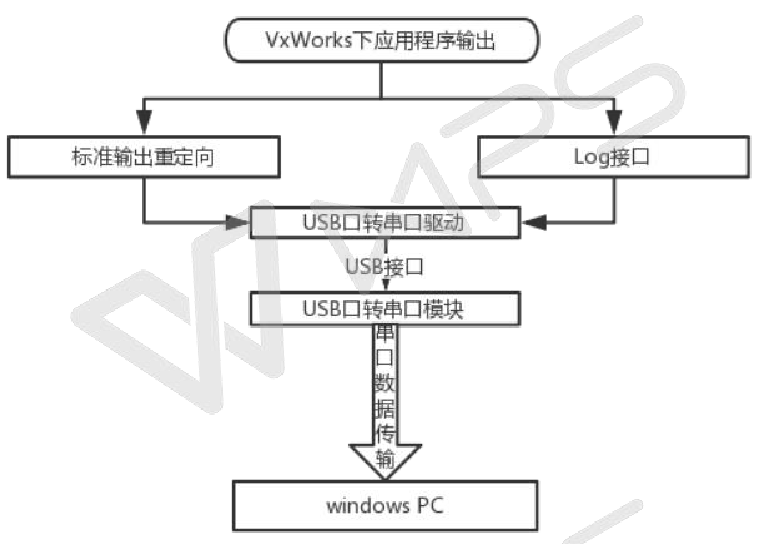
\includegraphics[width=.9\textwidth]{./graphics/debug-system-diagram.pdf}
\caption{调试通道整体结构图}\label{fig:debug-system-diagram}
\end{figure}
	
	整个调试通道主要分为两个模块:应用层的接口模块、USB口转串口模块。
	
	提供给应用层的接口模块负责将系统应用层的输出通过我们的USB口转串口驱动程序传输到windows PC机,输出的形式包括特定内容的格式化的输出和普通的重定向的输出,格式化的输出我们会使用自定义的Log接口进行格式控制,为此我们设计了一个自定义的Log协议格式,其中的内容包含有调试级别、调试信息所在的文件、调试信息所处的行号、输出该条调试信息的时间等;重定向的输出包括RTP模式下的重定向和task模式下的重定向,VxWorks中对于这两种模式需要使用不同的重定向方式。
	
	USB口转串口模块用于在VxWorks上实现一个USB口转串口驱动程序,负责将上层应用的信息传输到windows PC,包括一个特定需求的驱动程序的实现和一个普通的驱动程序的实现。特殊需求的驱动程序相对于普通的驱动程序而言在流程和结构上进行了修改,以使其达到特定的要求,具体的实现我们会在第三节进行介绍。两种实现方式中都会包含有驱动程序加载、卸载模块,设备的打开、关闭、读、写、控制模块。同时在驱动程序中还需要一个数据的管理模块,我们会使用循环缓冲区来管理数据。


\section{关键技术}

\subsection{VxWorks驱动开发}
	
	在VxWorks当中使用I/O子系统来管理设备驱动,I/O 子系统在整个VxWorks当中起着承上启下的作用,各种类型的设备都必须要向I/O子系统进行注册才能够被内核访问,I/O子系统在VxWorks当中的作用是维护系统设备表、系统驱动表、系统文件描述符表\cite{VxWorks内核解读}\cite{曹桂平2011VxWorks}。设备驱动在VxWorks中就靠这三个数据结构来进行管理,所以对于设备驱动而言非常重要。设备驱动程序初始化时会对硬件完成初始化的配置,同时会向I/O子系统注册自己,注册之后I/O子系统才能找到该驱动。

\subsubsection{VxWorks I/O 系统}
	通常操作系统为了应用程序的平台无关性都会为应用程序提供一套标准的接口,VxWorks也不例外,它为应用层的提供了接口函数有creat()、open()、unlink()、remove()、close()、rename()、read()、write()、ioctl()、lseek()、readv()、writev()等\cite{陈洋2007VxWorks}\cite{Wu2008Implementation}\cite{Zhang2010Design},我们通常将其称作为标准I/O 库函数。
	使用库函数可以在对应用层的程序进行开发和移植的时候使用同一套接口,这给应用程序的编程人员带来很大的方便,大大提高了其开发效率,避免了重复工作,而对于操作系统而言它需要通过调整底层驱动或者操作系统中间层来为标准I/O接口的实现提供支持。
	
	在Mac OS、Linux、或Windows当中会把这套接口以标准库的形式呈现,但是在VxWorks中它们是由系统的内核实现的,直接以内核文件的形式提供的,它们都位于ioLib.c文件下\cite{VxWorks内核解读}。之所以是以内核文件的形式来提供,是因为VxWorks当中不会区分用户态和内核态,这是VxWorks与通用操作系统的一个很大的不同点。在Vxworks当中所有的内核函数都可以不加限制的由用户程序直接进行调用,这样就减少了中断转入内核态再继续执行这一个过程,这对于强实时性系统而言极为重要,因为这样减少了时间开销,但是这样实现的一个缺点是减少了系统使用权限上的限制,为内核带来了很大的不安全性,极易导致内核的崩溃,所以VxWorks系统上应用程序的开发和使用对开发人员的要求比较高。
		
	VxWorks中I/O调用结构如\autoref{fig:I/O调用}所示。
	\begin{figure}[!h]
\centering
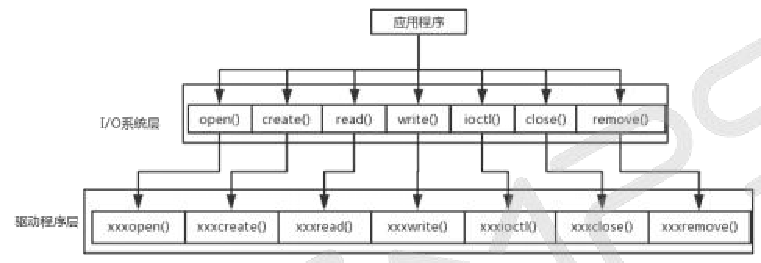
\includegraphics[width=1.0\textwidth]{./graphics/IOCall.pdf}
\caption{I/O调用}\label{fig:I/O调用}
\end{figure}

	
\subsubsection{系统设备表}
	系统设备表是VxWorks中为了管理系统上的所有设备而使用的一个链表,系统设备表中每一个节点都是一个DEV\_ HDR类型的结构体,系统会将每个设备DEV\_ HDR连接在如\autoref{fig:VxWorks系统设备示意图}所示的系统设备表中。DEV\_ HDR是wind内核规定的每一个设备都必须要具有的一个数据结构,且必须是设备自定义结构的第一个成员,之后系统只会使用这个结构来代表该设备。DEV\_ HDR结构体当中只包含有三个成员:一个设备链表节点;一个设备驱动号;一个指向设备名的指针。
	其定义如\autoref{fig:DEVHDR} 所示。

\begin{figure}[!h]
\centering
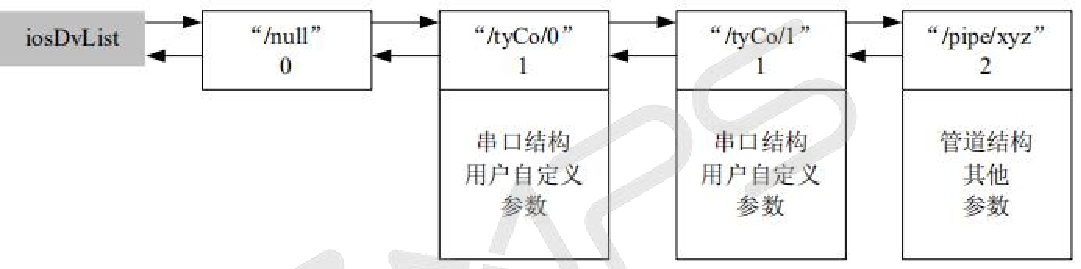
\includegraphics[width=1.0\textwidth]{./graphics/vxworks-device-link.pdf}
\caption{VxWorks系统设备示意图}\label{fig:VxWorks系统设备示意图}
\end{figure}
	
\begin{figure}[!h]
\centering
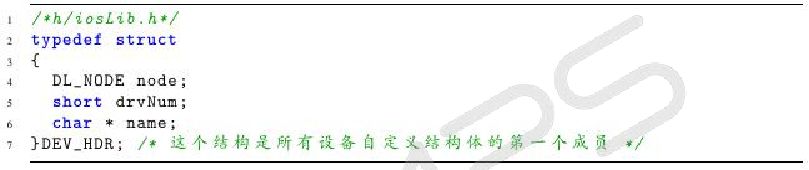
\includegraphics[width=1.0\textwidth]{./graphics/DEVHDR.pdf}
\caption{DEV\_ HDR结构体}\label{fig:DEVHDR}
\end{figure}

同时VxWorks系统提供了一个设备的注册函数iosDevAdd( DEV\_ HDR *pDevHdr, char *name, int drvnum),该函数用来将一个设备添加到系统设备表当中,系统设备表在每次添加设备时就会在表中增加一个节点表示该设备,删除设备时就会将该设备的节点从表中删除,一个设备添加到系统之后,就可以使用open()函数对其进行操作,open()会通过将传递过来的设备名与系统设备表当中进行设备名匹配来完成设备的打开操作,匹配的原则是最佳匹配,匹配成功之后就可以实现文件与设备的连接\cite{刘小军2008基于},之后就可以使用相对应的注册的设备驱动进行其他的文件操作。

\subsubsection{系统驱动表}	
	系统驱动表用于管理当前注册到I/O子系统下的所有驱动程序,既可以是直接驱动硬件工作的驱动程序,也可以是注册到I/O子系统下的驱动中间层\cite{VxWorks内核解读}。
	在VxWorks中系统驱动表的底层实现是一个数组,数组中的每一个元素就是一个系统驱动表的表项,每一个表项都是一个 DRV\_ ENTRY 类型的结构体,该结构定义在内核的头文件iosLibP.h当中,其定义如\autoref{fig:DEVENTRY}所示。
	
\begin{figure}[!h]
\centering
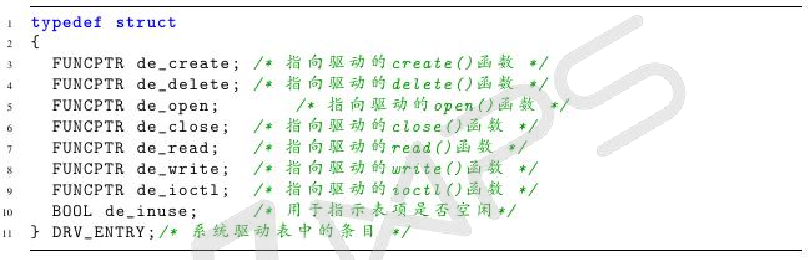
\includegraphics[width=1.0\textwidth]{./graphics/DEVENTRY.pdf}
\caption{DEV\_ ENTRY结构体}\label{fig:DEVENTRY}
\end{figure}

	DEV\_ ENTRY结构体当中的大多数成员都是函数指针,他们用于指向所注册的驱动程序中的一个用于完成特定功能的实际函数,这些函数的功能要符合IO系统预定义好的规则,这些函数被加入到系统驱动表中之后就可以完成与用户层提供的标准函数接口对接\cite{VxWorks内核解读}\cite{VxWorksDriverAPI}\cite{Wind2003VxWorks}。在DEV\_ ENTRY结构体当中唯一不是函数指针的成员是一个布尔类型的 de\_ inuse 成员,若该成员为FALSE则表示该表项目前是未被使用的状态,即该表项没有被任何的驱动所注册。

	VxWorks当中给我们提供了一个驱动的注册函数iosDrvInstall(),使用该函数注册我们的驱动之后,系统驱动表就会分配一个未被使用的表项给该驱动,然后使用iosDrvInstall()所提供的的参数来填充系统驱动表当中的指针,并将de\_ inuse置为TRUE的状态,一个驱动程序不需要实现所有的IO函数,对于实现的函数,在注册时直接将其指针置为NULL即可。


\subsubsection{系统文件描述符表}
	系统描述符表用于管理当前系统中所打开的所有文件描述符,VxWorks中系统描述符表的底层实现也是一个数组。每次执行open()调用成功之后,系统就需要从系统描述符表中分配一个表项给程序使用,并将文件描述符的表项索引作为文件描述符的ID返回给应用程序。之后应用程序直接通过这个ID就可以对文件进行操控,无需每次都是用文件名。
	在VxWorks中,标准输入、标准输出、标准错误输出虽然使用 0,1,2 三个文件描述符来表示,但是它在底层的实现上可能并不是占用了三个文件描述符表的表项,而是只占用一个表项,即三个文件描述符指向同一个文件描述符的表项\cite{VxWorks内核解读}\cite{An2003Implementation},这一点是需要注意的。
		
	
系统文件描述符表中每一个表项都使用 FD\_ ENTRY 这个结构体来表示,这个结构定义在内核的头文件iosLibP.h 中,其定义如\autoref{fig:FDENTRY}所示。


\begin{figure}[!h]
\centering
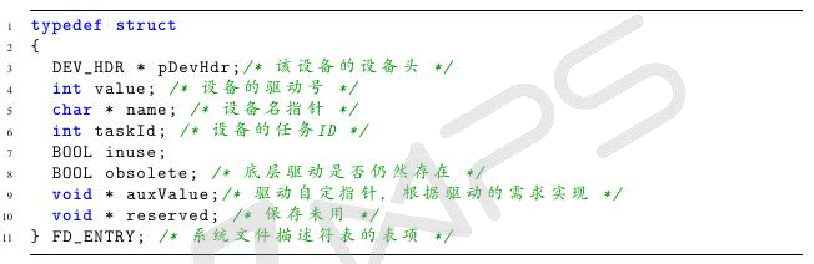
\includegraphics[width=1.0\textwidth]{./graphics/FDENTRY.pdf}
\caption{FD\_ ENTRY结构体}\label{fig:FDENTRY}
\end{figure}


用户的应用程序每次使用open()系统调用系统文件描述符表中就会增加一个有效表项,该表项的FD\_ ENTRY结构体会根据open()调用的内容来进行填充,每一个文件能够进行的open()调用是有限制的,因为数组的容量是固定的,每个驱动的FD\_ ENTRY结构数组满了之后就无法再对这个设备进行open()操作,此时 open()函数将会失败返回\cite{VxWorks内核解读}。系统会在表中的索引偏移 3 (0、1、2被系统占用)之后找一个最先找到的未使用的id作为文件描述符返回给用户。
	
\subsection{VxWorks 中的通信机制}
	
	任务间的通信机制用于协调多个任务之间的活动,在我们的USB口转串口驱动程序当中需要使用任务间的通信机制来确保对驱动内部缓冲区中的数据正确、有序的读写,VxWorks内核当中为我们提供了丰富的任务间通信机制,包括共享内存、信号量、消息队列、管道、信号、Sockets等。我们主要介绍一下VxWorks任务中使用较多的信号量、消息队列和管道这三种机制,它们在本质上都是使用的共享物理内存机制,只是这块共享的内存不是由用户进行管理,而是交由内核进行管理的,这种实现机制可以使任务间通信安全有序的进行\cite{胡明民2012基于实时操作系统}\cite{冯云贺2014基于}。

\\

\noindent \textbf{1. 信号量}
	
	信号量是一种在程序的设计当中最常使用的通信机制,其主要作用是线程间的同步和互斥。VxWorks中提供POSIX信号量的同时还设计了专门的wind信号量,POSIX信号量的使用主要是为了方便程序的移植。
	和POSIX信号量的不同之处在于,VxWorks中设计的wind信号量为VxWorks系统进行了高度的优化,使得其更适用于实时操作系统,能够更快的实现任务间通信。VxWorks中信号量是一个指向SEMAPHORE类型的结构指针,提供了二进制信号量、互斥信号量、计数信号量三种类型的信号量机制,他们适用于解决不同类型的问题。
	
\begin{itemize}
\item 二进制信号量\\
	二进制信号量是最快、最通用的信号量,既可以用于同步也可以用于资源计数。wind的二进制信号量所需系统开销最少,适用于高性能的需求。二进制信号量在资源可用时标记为FULL,在资源不可用时标记为EMPTY。在VxWorks中二进制信号量使用函数semBCreate()来创建,二进制信号量的提取和释放过程如\autoref{fig:二进制信号量的提取与释放过程} 所示。

\begin{figure}[h]
\centering
  \begin{subfigure}[b]{1.0\textwidth}
  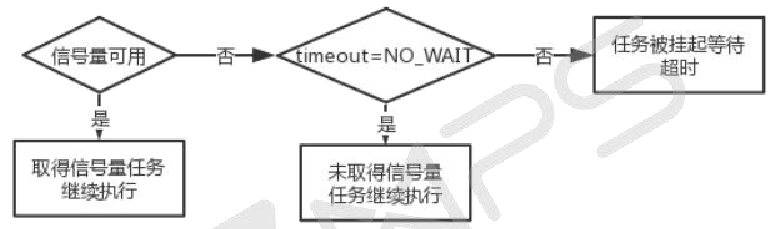
\includegraphics[width=\textwidth]{./graphics/erjinzhiTiQu.pdf}
  \caption{提取信号量}\label{fig:cp2102Front}
  \end{subfigure}
  ~
  \begin{subfigure}[b]{1.0\textwidth}
  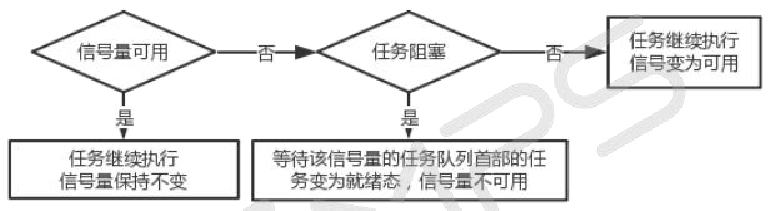
\includegraphics[width=\textwidth]{./graphics/erjinzhiShiFang.pdf}
  \caption{释放信号量}\label{fig:cp2102Rear}
  \end{subfigure}
\caption{二进制信号量的提取与释放过程}\label{fig:二进制信号量的提取与释放过程}
\end{figure} 


\item 互斥信号量\\
	互斥信号量可以看做是一种特殊的二进制信号量(资源数为1),它优化了互斥、优先级继承、删除安全等问题,这使得它能够更好的服务于任务间的互斥需求;互斥信号量的基本行为和二进制信号量是一致的,但是互斥信号量只能够用于互斥,不能够用于同步,该信号量只能够由获得的该信号量的进程来进行释放,不能够由其它的进程进行释放。它使用SEM\_ INVERSION\_ SAFE和SEM\_ Q\_ PRIORITY选项来使得该信号量能继承优先级算法,以此解决优先级的倒置问题;使用SEM\_ DELETE\_ SAFE选项来解决删除安全问题,在VxWorks中互斥信号量使用系统提供的semMCreate()函数来创建;
	
\item 资源计数信号量\\
	资源计数信号量也是一种特殊的二进制信号量(资源数较多),它会跟踪信号量增加、删除的次数,每次释放一个信号量,内部的计数器就会执行加一操作,每次提取一个信号量,内部的计数器就会执行减一操作,当计数器为0时,表示没有可供使用的资源,此时提取信号量的操作就会被阻塞,在VxWorks中资源计数信号量使用系统提供的semCCreate()函数来创建。

\end{itemize}
	
三种信号量的释放操作都是使用semGive()函数;提取操作都是使用semTake()函数,在提取信号量是我们可以选择是否允许超时,超时可以作为解决阻塞的一种方法。

	\\
	
\noindent \textbf{2. 消息队列}

	消息队列是一种在消息传输的过程中保存消息的容器,它给互相合作的任务间提供了一种通信机制。如\autoref{fig:消息队列}是消息队列实现任务间通信的一种方式。
	和信号量类似,VxWorks中也支持POSIX消息队列,其目的主要是为了方便移植和程序的兼容,同时VxWorks中也设计了专门用于Wind的消息队列,位于msgQLib文件当中。VxWorks中提供函数msgQCreate()来创建一个消息队列;msgQDelete()用于删除一个消息队列;msgSend()用于向消息队列中发送一个消息;masgQReveice()用于从消息队列中提取一个消息。
	
	在wind中消息队列是使用结构数组来实现的,在创建消息队列时必须指定一个消息的最大长度和队列中能够容纳的消息数量,这一特性使得其在任务间传递较多信息时存在的很大的局限性\cite{冯云贺2014基于}。
	
\begin{figure}[!h]
\centering
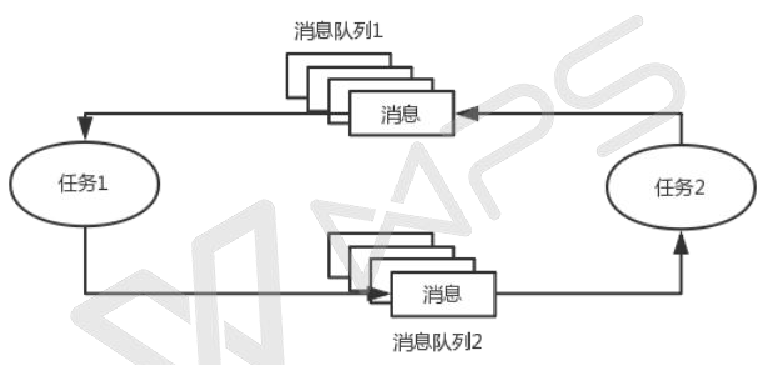
\includegraphics[width=0.9\textwidth]{./graphics/messageQueue.pdf}
\caption{消息队列实现全双工通信}\label{fig:消息队列}
\end{figure}	
				


\\	
	
	\noindent \textbf{3. 管道}
	
	管道也是一种基本的进程间通信机制,包括命名管道和匿名管道。VxWorks内核当中使用环形队列的方式来实现管道,管道提供了比消息队列更流畅的信息传递机制,可以像文件一样进行读写。命名管道具有一个与之关联的路径名,因此任何的进程间都可以用它进行通信,命名管道是双工的数据可以双向流动;非命名管道一般用于父子或兄弟进程间通信,非命名管道是半双工的,数据只能向一个方向流动。

\\
	
\noindent \textbf{4. 任务间特殊的通信机制--信号} 

	信号通常用于通知一个进程发生了异步事件,也被称为软中断。通常收到信号的进程通常可以选择三种方式来处理:一是使用一个信号处理函数处理;二是选择忽略该信号;三是使用系统默认的处理方式处理。
Wind内核同时支持UNIX BSD风格的信号和POSIX 信号,但是Vxworks中的信号处理机制有些特别之处,对于SIGKILL,SIGSTOP这类的信号,在通用操作系统上是不允许用户修改其默认处理函数的,但是在 VxWorks 操作系统中可以对任何信号的处理函数都可以进行更换的。



\subsection{USB技术}
	USB(Universial Serial Bus)作为PC领域的最新型的接口技术,目前已被各个PC厂家所支持,并且在各类外设当中都广泛的采用USB接口。USB的开发技术也已经很成熟,通用串行总线开发者论坛(USB Implementers Forum,USB IF)目前制定了三种USB接口标准:USB1.1,USB2.0和USB3.0。USB采用菊花链的形式连接所有的设备,最多可以连接127个设备,USB的总线拓扑结构如\autoref{fig:USB体系结构}所示
\begin{figure}[!h]
\centering
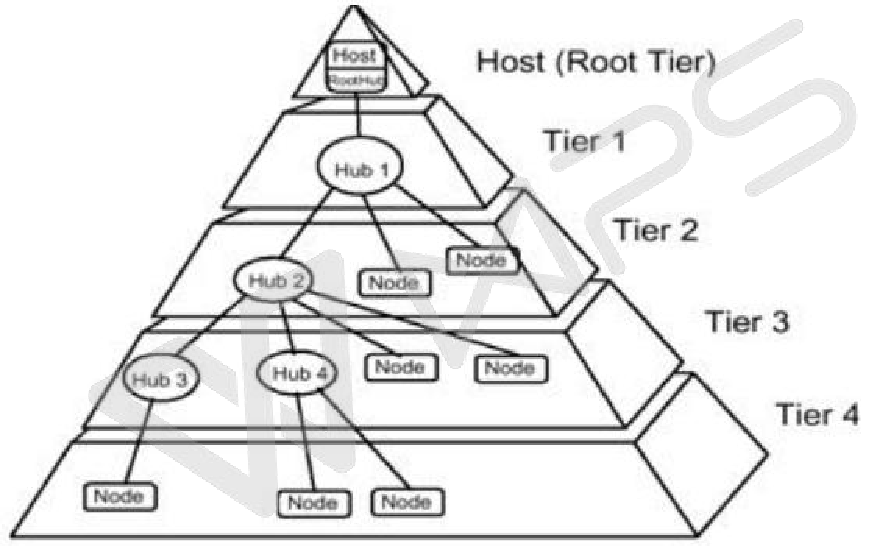
\includegraphics[width=1.0\textwidth]{./graphics/usb-structure.pdf}
\caption{USB总线拓扑结构}\label{fig:USB体系结构}
\end{figure}


USB的体系结构由三个部分组成,分别是USB主机(Host)、USB集线器(Hub)、USB设备(Device)。其中我们需要了解的关键部分是USB主机和USB设备。

\\
	
\noindent \textbf{1. USB主机}
	
	USB主机是USB体系中的核心,且系统中只允许一个USB主机存在。USB主机上的USB接口是USB主控制器,其控制着总线上所有USB设备数据通信。对于USB的体系结构而言,其数据的传输都是USB主机端发起的,非主机端(设备端)只能够被动的进行响应。USB主机需要完成的功能包括检测设备的热插拔、管理主机和设备之间的信息(控制和数据)流\cite{李雪红2004USB}\cite{莫宏伟2001USB}。


\\

\noindent \textbf{2. USB设备}

	USB设备指的是提供具体功能的而外部USB设备,是相对USB主机而言的,它们受USB主机的控制,只能对主机的请求进行被动响应。USB主机端会在检测到USB设备的动作之后会通过默认管道和USB设备进行通信,对其进行必要的初始化配置,并给设备提供适合的驱动程序(如果有的话),一个USB设备会通常会有很多的属性,它会通过这些属性来完成主机的配置要求。一些USB设备的属性如下:
	\begin{itemize}
	\item \textbf{描述符(Descriptor)属性}\\
	描述符是USB协议中定义的一套用来描述USB设备的功能和属性的固定结构,我们可以通过描述符了解设备的各种属性,描述符又分为设备描述符、配置描述符、接口描述符、端点描述符、字符串描述符\cite{张杰2008基于}\cite{边海龙2004USB}除此之外,设备还可以提供自己专用的描述符,分为设备类描述符和供应商自定义描述符,我们使用的USB口转串口设备就不属于一个标准的USB设备,它会为我们提供供应商自定义的描述符,我们使用需要使用它来对设备进行识别。
	
	\item \textbf{类(Class)属性}\\
	由于USB协议支持许多的外围设备,而这些设备又可以根据功能来分成一些相近的类,如打印机类、键盘类等。这样主机端就可以为这些功能相近的设备提供一个类驱动,类驱动可以用于驱动所有属于同一类的设备,不需要再为每一个设备提供一个完整的驱动程序。这大大的方便的设备的制造商,他们的设备只需要符合某一类的驱动,就可以使用该类驱动程序来驱动其设备,之后只需要实现简单的包含有设备特性的客户端驱动即可,若设备没有特殊的特性,则直接使用类驱动即可\cite{李雪红2004USB}。	
	
	\item \textbf{功能(Function)/接口(Interface)属性}\\
	功能或接口是USB协议中定义的设备的某种能力,Function是从功能角度来说的,从设备的角度来说,被称为Interface。对于一个设备他可以拥有很多个不同的接口,每一个接口负责完成设备的一个特定的功能,并且这个接口具体实现什么样的功能并不是固定的,当USB设备处于可配置状态的时候能够通过控制命令来改变某一个接口的功能,一个接口能够具有什么样的功能会在USB的接口描述符中进行描述。
	
	\item \textbf{端点(Endpoint)属性}\\
	端点是USB设备与USB主机逻辑上的通信流的终点,每个设备都拥有一个可独立进行操作的端点集合,且每个端点在使用时都要先初始化其数据传输方向(IN/OUT),即使端点号相同但是传输方向不同的通信点也是不同的端点\cite{李雪红2004USB}。
	
	\item \textbf{管道}\\
	管道可以看做是设备上的一个端点和主机上的软件的联合体,设备和主机间的数据传输要基于管道进行。在USB的通信过程中首先要建立一个管道才能够进行数据的传输,USB设备在和主机通信时都会建立一个默认的管道,这个管道对应的端点是默认端点0,之后需要自己使用其它的端点来建立我们的数据传输过程中需要使用的输入或输出管道。在我们的USB口转串口驱动中会为每一个设备建立两个管道,一个批量输出管道和一个批量输入管道。
	
	\item \textbf{设备地址}\\
	设备地址用于区分USB系统中的一个USB设备的特殊标识,设备地址会在设备初始化之后由主机进行分配且是唯一的。设备地址单元共有7bit,其中地址0是缺省地址,在设备初始化的时候使用,理论上系统可以区分127个USB设备\cite{李雪红2004USB}。
	\end{itemize}	



\noindent USB规范规定了USB主从设备之间的四种传输方式,每种方式有各自的用途\cite{USB总线接口开发指南}:

\begin{itemize}
\item \hei{控制传输}:控制传输USB传输方式中最重要、最复杂的一种,它适用于少量、对时间和速率无要求的场合,一个USB设备插入主机之后就是使用这种传输方式来读取设备的地址和描述符等信息。所有的设备都会在其0号端点的缺省管道当中支持控制传输\cite{张杰2008基于}。
\item \hei{批量传输}:批量传输有两种最基本的事物类型:BULK\_ IN和BULK\_ OUT,其主要用于处理对数据传输速率不是很高的情况,批量传输使我们的USB口转串口设备所使用的主要传输传输方式,每次有数据需要传输时我们都会构建一个IRP使用批量传输将其传出或传入。
\item \hei{中断传输}:中断传输也有两种基本的事务:IN和OUT,其主要是为那些要快速实现主机和设备的交互,但是数据量很小、对服务时间有要求的情况而准备的。
\item \hei{等时传输}:等时传输也是由基本的IN和OUT两种事务组成,主要用于处理大量、恒速、对时间周期有要求的数据。等时传输只有全速和高速设备才支持,低速设备不支持\cite{张杰2008基于}。
\end{itemize}


	

\section{本章小结}
	本章重点介绍了本次的VxWorks调试通道的整体架构,并介绍了介绍了各个部分的设计方案,最后介绍了在本次的设计当中所需要使用关键技术和所需了解的重要知识,主要包括VxWorks下的驱动开发必须的结构、驱动中所需使用的VxWorks的通信机制、缓冲区技术、USB技术。下面将要讨论VxWorks下的调试通道的详细的设计细节和具体的实际机制。



























%\subsection{第二层}\label{sec:1}
%\subsubsection{第三层}\label{sec:1}
%测试测试测试测试测试测试测试测试测试测试测试测试。
%\footnote{\label{footnote:1}脚注}

\section{字体}

普通\textbf{粗体}\emph{斜体}

\hei{黑体}\kai{楷体}\fangsong{仿宋}

\section{公式}

单个公式,公式引用:\autoref{eq:1}。
\begin{equation}
 c^2 = a^2 + b^2 \label{eq:1}
\end{equation}

多个公式,公式引用:\autoref{eq:2},\autoref{eq:3}。

\begin{subequations}
\begin{equation}
  F = ma \label{eq:2}
\end{equation}
\begin{equation}
  E = mc^2 \label{eq:3}
\end{equation}
\end{subequations}

\section{罗列环境}

\begin{enumerate}
    \item 第一层\label{item:1}
    \item 第一层
    \begin{enumerate}
        \item 第二层\label{item:2}
        \item 第二层
        \begin{enumerate}
            \item 第三层\label{item:3}
            \item 第三层
        \end{enumerate}
    \end{enumerate}
\end{enumerate}

\begin{description}
    \item[解释环境]  解释内容
\end{description}



\clearpage
\chapter{实时操作系统VxWorks}
\section{概述}
\subsection{实时操作系统}
实时操作系统(Real Time Operation System)是整个实时系统的核心。POSIX1003.1标准为RTOS下了一个简单的定义:RTOS是能够在有限的响应时间内为应用提供所要求级别服务的操作系统\cite{Renard20081003}。这个系统能够对任何时间要求苛刻的事件服务,能够在正确的时间内做正确的事情。实时系统按照实时的效果可以分为软实时和硬实时,一个好的实时操作系统能够使你的系统时钟满足要实现的需求,即使在系统的负荷很重的情况下。

现代实时操作系统基于多任务和任务间通信的互补概念。多任务环境允许将实时应用程序构建为一组独立任务,每一个任务都有自己的执行线程和一组系统资源。任务间通信设施允许这些任务同步并进行协调其活动。在VxWorks中,任务间通信工具从快速信号量到消息队列,从管道到网络透明套接字。

	实时系统的另外一个关键设施是硬件中断处理,因为中断处理时通知系统发生外部时间的常用机制。为了尽可能快地响应中断,VxWorks中的中断服务例程(ISR)运行自己的特定上下文中,这个上下文在任何其他的任务上下文之外\cite{Wind2003VxWorks}。

操作系统的核心是内核。内核控制着计算机系统上的所有硬件和软件资源,在必要的时候给应用程序分配硬件资源,并执行相应的操作命令。

	内核的主要功能为以下的四种:

\bullet 系统的内存管理:不仅可以管理服务器上的可用物理内存,还可以创建和管理虚拟内存。

\bullet 软件程序管理:内核控制着系统上运行着的所有程序。

\bullet 硬件设备管理:任何需要操作系统与之进行通信的设备都需要在内核的代码当中加入其驱动程序代码。驱动程序代码相当于应用程序和硬件设备间的中间人,允许内核和设备之间交换数据。

\bullet 文件系统管理:不同于其他的一些操作系统,Linux内核支持通过不同类型的文件系统从硬盘当中读写数据。除了自有的诸多文件系统之外,Linux还支持从其他的操作系统(如windows)采用的文件系统中读写数据。内核必须在编译时就加入对所有可能用到的文件系统的支持。Linux内核采用虚拟文件系统(Virtual File System,VFS)作为和每一个文件系统交互的接口。这为Linux内核同任何类型文件系统通信提供了一个标准的接口,当每个文件系统都被挂载和使用时,VFS将信息都缓存在内存当中。

VxWorks是一种基于微内核技术的实时操作系统。


\section{代码环境}

\begin{lstlisting}[language=python]
import os

def main():
    '''
    doc here
    '''
    print 'hello, world' # Abc
    print 'hello, 中文' # 中文
\end{lstlisting}

\section{定律证明环境}

\begin{definition}\label{def:1}
这是一个定义。
\end{definition}
\begin{proposition}\label{proposition:1}
这是一个命题。
\end{proposition}
\begin{axiom}\label{axiom:1}
这是一个公理。
\end{axiom}
\begin{lemma}\label{lemma:1}
这是一个引理。
\end{lemma}
\begin{theorem}\label{theorem:1}
这是一个定理。
\end{theorem}
\begin{proof}\label{proof:1}
这是一个证明。
\end{proof}

\section{算法环境}

\begin{algorithm}[H]
\SetAlgoLined
\KwData{this text}
\KwResult{how to write algorithm with \LaTeX2e }
initialization\;\label{alg_line:1}
\While{not at end of this document}{
read current\;
\eIf{understand}{
go to next section\;
current section becomes this one\;
}{
go back to the beginning of current section\;
}
}
\caption{How to write algorithms}\label{alg:1}
\end{algorithm}

\section{表格}
表格见\autoref{tab:1}。

\begin{table}[!h]
\centering
\caption{一个表格}\label{tab:1}
\begin{tabular}{|c|c|}
\hline
a & b \\
\hline
c & d \\
\hline
\end{tabular}
\end{table}
\section{图片}
图片见\autoref{fig:1}。图片格式支持eps,png,pdf等。多个图片见\autoref{fig:2},分开引用:\autoref{fig:2-1},\autoref{fig:2-2}。

\begin{figure}[!h]
\centering
\includegraphics[width=.4\textwidth]{fig-example.pdf}
\caption{一个图片}\label{fig:1}
\end{figure}

\begin{figure}[!h]
\centering
  \begin{subfigure}[b]{0.3\textwidth}
  \includegraphics[width=\textwidth]{fig-example.pdf}
  \caption{图片1}\label{fig:2-1}
  \end{subfigure}
  ~
  \begin{subfigure}[b]{0.3\textwidth}
  \includegraphics[width=\textwidth]{fig-example.pdf}
  \caption{图片2}\label{fig:2-2}
  \end{subfigure}
\caption{多个图片}\label{fig:2}
\end{figure}

\section{参考文献示例}
这是一篇中文参考文献\cite{徐媛媛2003嵌入式实时操作系统的设备驱动};这是一篇英文参考文献\cite{9787508342894};同时引用\cite{9780124467422,bamboosilk}。

\section[\textbackslash{}autoref 测试]{\texttt{\textbackslash{}autoref} 测试}

\begin{description}
  \item[公式] \autoref{eq:1}
  \item[脚注] \autoref{footnote:1}
  \item[项] \autoref{item:1},\autoref{item:2},\autoref{item:3}
  \item[图] \autoref{fig:1}
  \item[表] \autoref{tab:1}
  \item[附录] \autoref{appendix:1}
  \item[章] \autoref{chapter:1}
  \item[小节] \autoref{sec:1},\autoref{sec:2},\autoref{sec:3}
  \item[算法] \autoref{alg:1},\autoref{alg_line:1}
  \item[证明环境] \autoref{def:1},\autoref{proposition:1},\autoref{axiom:1},\autoref{lemma:1},\autoref{theorem:1},\autoref{proof:1}
\end{description}

% backmatter用于表示论文的正文结束
\backmatter

%ack 环境用于致谢页面
\begin{ack}
致谢正文。
\end{ack}

% bibliography用于生成参考文献。
\bibliography{ref/myref.bib}

% appendix环境用于附录环境。即可以将附录置于appendix环境当中。如:
% \begin{appendix}
%  <content>
% \end{appendix}

% 直接使用\appendix 则表明后文均为附录。如:
% \appendix
%  <content> 
\appendix

% publications环境用于已经发表了的论文的页面,一般用于附录当中,使用上同enumerate环境
\begin{publications}
    \item 论文1
    \item 论文2
\end{publications}

\chapter{这是一个附录}\label{appendix:1}
附录正文。


\end{document}

\endinput
%%
%% End of file `hustthesis-zh-example.tex'.
